\documentclass[t]{beamer}
\usetheme{Copenhagen}
\setbeamertemplate{headline}{} % remove toc from headers
\beamertemplatenavigationsymbolsempty

\usepackage{amsmath, array, tikz, bm, pgfplots, tcolorbox, graphicx, venndiagram, color, colortbl, xfrac}
\pgfplotsset{compat = 1.16}
\usepgfplotslibrary{statistics}
\usetikzlibrary{calc}

\title{Hypothesis Testing}
\subtitle{Single Sample Mean}
\author{}
\date{}

\AtBeginSection[]
{
  \begin{frame}
    \frametitle{Objectives}
    \tableofcontents[currentsection]
  \end{frame}
}

\begin{document}

\pgfmathdeclarefunction{gauss}{2}{%
  \pgfmathparse{1/(#2*sqrt(2*pi))*exp(-((x-#1)^2)/(2*#2^2))}%
}

\begin{frame} 
\maketitle
\end{frame}

\begin{frame}{Student's $t$ Test}
While the $z$ test for a population mean may be a good introduction to hypothesis testing, it doesn't hold much use in the real world. \newline\\	\pause

After all, how likely is it that you know for certain what the population standard deviation, $\sigma$, is, but you still have doubts about the population mean?	\newline\\	\pause

William Sealy Gosset, under the pseudonym \textit{Student}, created a hypothesis test for the population mean when the population standard deviation is unknown.
\end{frame}

\begin{frame}{Assumptions for Using the $t$ Test for a Population Mean}
\textbf{Assumptions:} 
\begin{itemize}
	\item<2-> The sample come from a normally distributed population; especially important for small sample sizes
	\item<3-> Sample was obtained randomly
\end{itemize}
\end{frame}

\begin{frame}{Degrees of Freedom}
The \textbf{degrees of freedom} of a sample size $n$ is given as $n - 1$.	\pause

\begin{center}
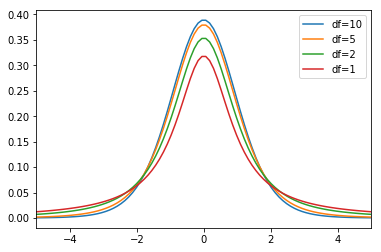
\includegraphics[scale=0.6]{../Images/t_distribution_df.png}
\end{center}
\pause

As the degrees of freedom grow, the $t$ distribution becomes more normal.
\end{frame}

\begin{frame}{Summary Stats}
Similar to a $z$ score, the test statistic $t$ can be found by calculating
\[t = \frac{\overline{x}-\mu}{s/\sqrt{n}}\]
\pause
$p$-value can be calculated using the test statistic and area under the curve. \newline\\	\pause
Confidence intervals for $t$ distribution are given by
\[\overline{x} \pm t_{\alpha/2}\left(\frac{s}{\sqrt{n}}\right)\]
where the degrees of freedom help determine the value of $t_{\alpha/2}$
\end{frame}

\begin{frame}{Am I Going to Be OK With This?}
If you understood the concepts and ideas behind the hypothesis testing we've done (in particular, being able to work with test statistics and critical values, $p$-values, or confidence intervals) then you should be alright with this section.	\newline\\	\pause

Quite frankly, just about all of the remaining material regarding hypothesis testing is just a variation on that theme.		\newline\\	\pause

Remember, most modern statistics uses computers or other technology to crunch the numbers. \newline\\	\pause

In the grand scheme of things, it's more valuable to be able to \emph{interpret those results}.
\end{frame}

\begin{frame}{Example 1}
A car company claims one model of their SUV gets 40 mpg. You want to test the claim that the mean mpg of this model of SUV is less than 40 mpg, so you obtain a random sample of 65 of these cars and find the sample mean is 39 mpg with a standard deviation of 5.1 mpg. Test your claim at the $\alpha = 0.05$ significance level.	\newline\\	\pause

$H_0: \, \mu = 40$ mpg	\newline
$H_A: \, \mu < 40$ mpg
\end{frame}

\begin{frame}{Example 1}
The critical value corresponding to $\alpha=0.05$ of a left-tailed test is $-1.669$. \newline\\	\pause

$t = -1.581$ \newline
$p$-value = 0.0594	\newline
95\% upper bound: 40.0558  \newline (we are 95\% confident the population mean is 40.0558 or less)\newline\\	\pause

Do not reject the null hypothesis.	\newline\\ \pause
\begin{quote}
At the 95\% confidence level, we do not have sufficient evidence to reject the claim that the mean mpg of this model SUV is 40 mpg, and conclude that our sample did not give us reason to believe the mean mpg might be less than 40.
\end{quote}
\end{frame}

\begin{frame}{Example 2}
A company claims it can boost your statistics grade by 10\%. You want to test the claim that the mean grade increase is not 10\%, so you randomly sample 20 statistics students who used the program and recorded their percent grade increase from one test to the next. Test your claim at the $\alpha = 0.1$ level of significance. \newline\\

\begin{center}
\begin{tabular}{ccccc}
8 & 5 & 7 & 9 & 10 \\
12 & 7 & 8 & 11 & 15 \\
4 & 13 & 9 & 8 & 11 \\
9 & 3 & 5 & 8 & 12 \\
\end{tabular}
\end{center}
\pause

$H_0: \, \mu = 10$ \\
$H_A: \, \mu \neq 10$
\end{frame}

\begin{frame}{Example 2}
The critical values corresponding to $\alpha = 0.1$ of a left-tailed test are $-1.729$ and 1.729.	\newline\\	\pause

$t = -1.877$	\newline
$p$-value = 0.0759 \newline
90\% confidence interval: (7.5027, 9.8973)	\newline\\	\pause

Reject the null hypothesis	\newline\\	\pause
\begin{quote}
At the 90\% confidence level, we have sufficient evidence to reject the claim that the mean increase in score is 10\% and conclude that our sample gives us reason to believe the mean increase in score is not 10\%.
\end{quote}
\end{frame}

\end{document}